%%%%%%%%%%%%%%%%%%%%%%
\documentclass{singlecol-new}
%%%%%%%%%%%%%%%%%%%%%%

\usepackage{natbib,stfloats}
\usepackage{mathrsfs}

%
\usepackage{amssymb}
\setcounter{tocdepth}{3}
\usepackage{graphicx}
%\usepackage{url}
\usepackage{amsmath}
\usepackage{amsfonts}
\usepackage{algorithm,algorithmic}
\renewcommand{\algorithmicrequire}{\textbf{Input:}}
\renewcommand{\algorithmicensure}{\textbf{Output:}}
\newcommand{\SWITCH}[1]{\STATE \textbf{switch} (#1)}
\newcommand{\ENDSWITCH}{\STATE \textbf{end switch}}
\newcommand{\CASE}[1]{\STATE \textbf{case} #1\textbf{:} \begin{ALC@g}}
\newcommand{\ENDCASE}{\end{ALC@g}}
\newcommand{\CASELINE}[1]{\STATE \textbf{case} #1\textbf{:} }
\newcommand{\DEFAULT}{\STATE \textbf{default:} \begin{ALC@g}}
\newcommand{\ENDDEFAULT}{\end{ALC@g}}
\newcommand{\DEFAULTLINE}[1]{\STATE \textbf{default:} }
\usepackage{hyperref}

\usepackage{listings}
\usepackage{xcolor}
\usepackage{booktabs}
\usepackage[tight,footnotesize]{subfigure}
%

\def\newblock{\hskip .11em plus .33em minus .07em}

\theoremstyle{TH}{
\newtheorem{lemma}{Lemma}
\newtheorem{theorem}[lemma]{Theorem}
\newtheorem{corrolary}[lemma]{Corrolary}
\newtheorem{conjecture}[lemma]{Conjecture}
\newtheorem{proposition}[lemma]{Proposition}
\newtheorem{claim}[lemma]{Claim}
\newtheorem{stheorem}[lemma]{Wrong Theorem}
%\newtheorem{algorithm}{Algorithm}
}

\theoremstyle{THrm}{
\newtheorem{definition}{Definition}[section]
\newtheorem{question}{Question}[section]
\newtheorem{remark}{Remark}
\newtheorem{scheme}{Scheme}
}

\theoremstyle{THhit}{
\newtheorem{case}{Case}[section]
}

\makeatletter
\def\theequation{\arabic{equation}}

\JOURNALNAME{\TEN{\it Int. J. Web and Grid Services,
Vol. \theVOL, No. \theISSUE, \thePUBYEAR\hfill\thepage}}%

\def\BottomCatch{%
\vskip -10pt
\thispagestyle{empty}%
\begin{table}[b]%
\NINE\begin{tabular*}{\textwidth}{@{\extracolsep{\fill}}lcr@{}}%
\\[-12pt]
Copyright \copyright\ 2016 Inderscience Enterprises Ltd. & &%
\end{tabular*}%
\vskip -10pt%
%\vskip -35pt%
\end{table}%
}

\makeatother

\begin{document}%
%%%%%%%%%%%%%%%%%

\title{Toward an Aspect-oriented Cache Autoloading Framework with Annotation}

\begin{abstract}
In recent years, researches focus on addressing the query bottleneck issue using data cache in the Internet-of-Things. However, the challenges of this method are how to implement autonomous management of data cache. In this paper, we propose an aspect-oriented cache autoloading framework (ACALFA). The architecture, annotation, expression are introduced to address cache auto load. There are some features for improving performance, such as load waiting, autoloading, loose coupling, and batch delete of cache. The result of experiments indicated that our approach is nearly 25\% faster than other cache frameworks in the scenario that data size is enormous and concurrency is very high.
\end{abstract}

\KEYWORD{Big Data; Data Cache; Aspect-Oriented Programming; Annotation; Pointcut; Grid Services.}

\maketitle


\section{Introduction}
\label{Introduction}

\subsection{Background}
Internet-of-Things (IoT) \cite{zanella2014internet} devices, connected to each other, will generate large-scale data such as weather monitoring data over a relatively short period of time. The real-time IoT data also brings significant challenges for data access and storage \cite{kaisler2013big}. For an optimization, the content routers such as Machine-to-Machine (M2M) gateways in the Internet can cache these results without relaying user requests all the way to data sources. The idea is similar to Content Delivery Network (CDN) of Web pages and multimedia files. However, these systems face cache penetration in the case of high concurrency \cite{nishtala2013scaling}.

Cache is a collection of data duplicating original values stored in memory, usually for easier access. Moreover, it can reduce the server response time efficiently \cite{ma2017segment}. There are many ways to implement the cache, such as the cache based on browser, the cache based on CDN \cite{manjhi2005finding} and the cache based on applications \cite{wu2011characterization}. Relative Database Management Systems (RDBMSs) combined with the NoSQL databases is the primary solution for the cache based on server, RDBMSs are used for data persistence, in-memory NoSQL databases are used for caching.

There are a lot of caches, but they all have some shortcomings. Current cache frameworks have some shortcomings. First, their expire policies have not particular optimization for the data that high-frequent access or need a long time to be processed. When the data concentrated is expired, a cache avalanche issue occurred, in case all requests foster together. This case might lead to the instability of the server \cite{ma2017column}. Second, cache logic and business logic are tightly coupled. It leads to cumbersome cache operations and is difficult for developers to maintain the cache data. Third, the cache may cause namespace conflict using distributed key-value database like Redis cluster.

\subsection{Contributions}
In this paper, we propose an aspect-oriented cache auto load framework with annotation. Contributions of our framework are concluded as follows.

\begin{itemize}
  \item Avoid cache breakdown and cache penetration using load waiting and autoloading. Autoloading can implement hot-spot data pre-loading. The cache work because the data can be obtained from memory and cut down the read back of source. To further reduce the read back of source, we can make the hot-spot data lurk in memory constantly and update it regularly. Moreover, the data that need to a long time to process also benefit from this strategy, system can load them before peak coming. Load waiting can reduce the server pressure when load data from database. Once the cache miss, there are many requests flowing into the database, but for the same data. Load wait strategy select a leader to request the data, others wait until the data are provided by the leader.
  \item Loose coupling of business and cache logic using AOP. The purpose of AOP is proposed to decrease the costs of cache maintenance.
  \item Batch delete of cache. It is inevitable that it leads the inconsistency of physical database and cache data. It is difficult to restore the key of the related cache by programs if the query statement is involved. Therefore, the precise batch delete of cache is proposed using hash tables. When this cache need to be removed, the system will remove the record of corresponding hash table directly.
\end{itemize}

\subsection{Organization}
The remainder of the paper is organized as follows. The current work of cache framework is discussed in Section \ref{RelatedWork}. In Section \ref{Framework}, aspect-oriented cache autoloading framework with annotation (ACALFA) is proposed. Architecture, annotation, expression of the aspect-oriented cache auto load framework are introduced. In Section \ref{Experiments}, the response time, cache improvement and pressure experiments show that our framework are effective and efficient. Brief conclusions and future research directions are outlined in the last section.


\section{Related Work}
\label{RelatedWork}

\subsection{Cache Framework}
Caching of data with weak consistency can achieve transparency. Typically, the cache content is periodically refreshed. There are different levels for caching performance, namely the browser cache \cite{davison2001web}, proxy cache \cite{kumar2008new}, Content Delivery Network (CDN) cache \cite{vakali2003content}, and server level cache \cite{ma2017column}. Browser cache is closest to the end user and can speed up page loads by storing the static files, such as a single page, on user's local storage media \cite{mookerjee2002analysis}. CachePortal \cite{candan2001enabling} relies on timestamps and HTTP logs to conservatively determine which pages to invalidate. It has a unique form of weak, time-lagged consistency. Proxy caches are situated at network access points for web users \cite{kumar2008new}. Consequently, proxy caches can store documents and directly serve requests for them in the network, thereby avoiding repeated traffic to web servers. CDN is similar to proxy caching \cite{vakali2003content}. But the difference is that the servers of CDN are distributed around the users, data is obtained from the server with least delay. The disadvantage of CDN cache is that excessive consumption of resources due to continuous analysis. Proxy cache and CDN solves the problem of the local cache cannot be shared. Although some of these products implement dynamic page cache, the effects are not good. In particular, server data processing efficiency is not effectively improved. Therefore, the present mainstream of cache is server level cache.

Recently, there are some new cache frameworks. The combination of RDBMSs and in-memory NoSQL is the mainstream architecture of server cache. Several solutions are proposed such as Redis \cite{zawodny2009redis}, Memcached \cite{hafeez2017realizing}, and EhCache. RDBMSs are used to persist data, and in-memory databases are used to store high-frequency data \cite {ma2017column}. Redis performs better for high concurrency and memory consumption. As an improvement, Memcache pool is used to duplicate high-frequency data into a dedicated data pool by cache access frequency and cache expired cost \cite{nishtala2013scaling}. This feature is achieved by the time of the cache analysis by some dedicated servers.

There are some optimizations of cache frameworks. For example, the performance of distributed storage with disks is studied \cite{scheuermann1998data}. Another data-aware cache framework (Dache) using MapReduce is proposed \cite{zhao2014dache}. In Dache, tasks submit their intermediate results to the cache manager. A task queries the cache manager before executing the actual computing work. The cache manager of ACALFA is a general framework that supports these cache frameworks.

\subsection{Aspect-Oriented Programming}
Aspect-Oriented Programming (AOP) is a programming methodology for separating crosscutting concerns \cite{kiczales2001aspect}. This method encapsulates behaviors that affect multiple classes into reusable modules \cite{ma2013toward}. By weaving rules specified by the developer, aspects are incorporated to form the final system. In this paper, we attempt to use this method to intercept cache events to implement the separation of cache from the business.

The key difference between AOP and other approaches is that AOP provides component and aspect languages with different abstraction and composition mechanisms \cite{pinto2017lara}. A special language processor called an aspect weaver is used to coordinate the co-composition of the aspects and components. Modularized crosscutting concerns are called aspects. An aspect, if it can not be cleanly encapsulated in a generalized procedure. AOP distinguishes between two approaches. Static crosscutting affects the static type signature of a program, whereas dynamic crosscutting allows to intercept a program at well-defined points in its execution trace. After evaluating the flexibility of the monitoring system, we decided to pursue dynamic crosscutting option over ease of implementation.

We adopt aspect-oriented programming techniques to manage the data cache. The capabilities of AOP in terms of isolating the aspect code from the source code of the used server make it a non-invasive caching approach.

\section{Aspect-oriented Cache Auto Load Framework with Annotation}
\label{Framework}

\subsection{Architecture}

\subsubsection{Overview}

\begin{figure} [htb]
\centering
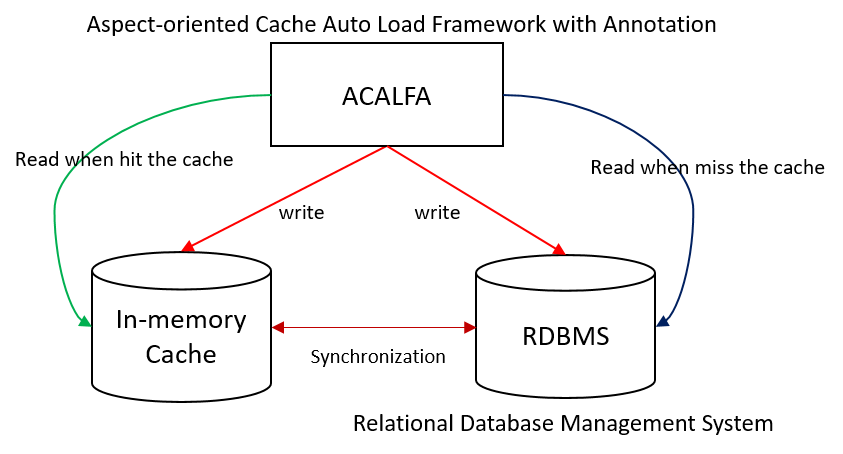
\includegraphics[width=1.0\linewidth]{img/architecture}
\caption{\label{architecture}Architecture of aspect-oriented cache auto load framework with annotation (ACALFA).}
\end{figure}

Figure \ref{architecture} gives the architecture of our proposed aspect-oriented cache auto load framework with annotation (ACALFA). ACALFA reads data from in-memory database when it hits the cache, while reads data from relational database management system (RDBMS) when it misses the cache. ACALFA writes data to both in-memory cache and RDBMS. They synchronize the data with each other. This framework is used to reduce the load of reading/writing service of big data applications. Load waiting and auto loading strategy is achieved by decreasing the concurrency number of read back of source RDBMS.

\begin{figure} [htb]
\centering
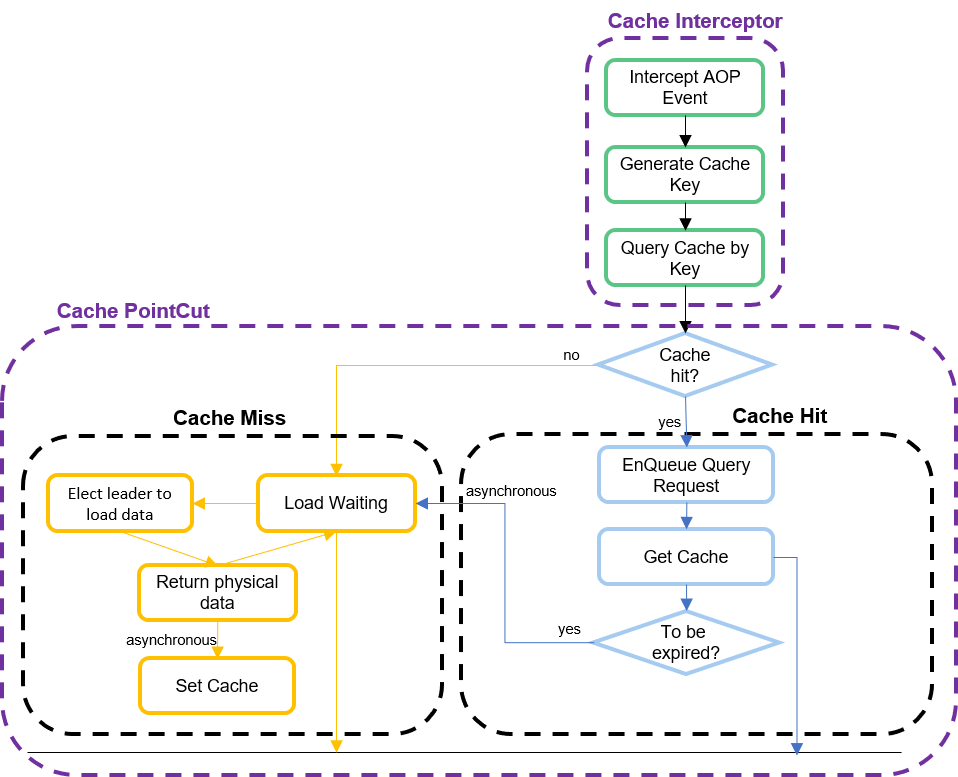
\includegraphics[width=1.0\linewidth]{img/process}
\caption{\label{process}Data processing of aspect-oriented cache auto load framework with annotation (ACALFA).}
\end{figure}

Figure \ref{process} shows the data processing of aspect-oriented cache auto load framework with annotation (ACALFA). Using aspect-oriented thinking, cache framework is loosely coupled with business and cache logic. Cache interceptor is used to intercept before/after the execution of business method, then generate the cache key by annotation to trigger cache query. Cache entry is triggered by custom cache events and its corresponding handler. Annotation, a form of metadata, provides data about a program that is not part of the program itself. Cache annotation is used to describe the point cut (cache logic) of our cache framework. It includes cache key, expire time, and cache type. The data of the in-memory cache is loaded by a unique cache key. Cache key is created by the expression in annotation dynamically.

\begin{figure} [htb]
\centering
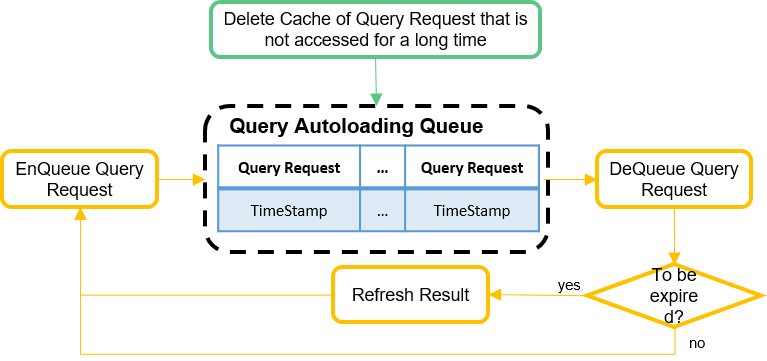
\includegraphics[width=1.0\linewidth]{img/autoloading}
\caption{\label{autoloading}Management of the query autoloading queue.}
\end{figure}

We design the processing of cache hit and miss shown in Figure \ref{process}. When the query hits the query, we put the query request to an autoloading queue for cache self management. If the cache result will be expired, it will trigger an asynchronous update of this cache. Figure \ref{autoloading} shows the management of the query autoloading queue. Cache-context message is recorded in the autoloading queue, including the query request and timestamp. A local thread monitors the autoloading queue to delete the corresponding cache of the query request that is not accessed for a long time. Autoloading queue guarantees the hot spot data is resident in memory. A maximum queue length limit is set to control the capacity.

When the query misses the query, the cache framework will asynchronously elect a leader to load data from physical database. Loading waiting can avoid cache breakdown under high concurrency. That is to say that a large number of query requests with the same key in cache miss will not cause large amount of read back of source physical database.

\subsubsection{Implementation}
There are several components to implement ACALFA:

\begin{itemize}
    \item $CacheInterceptor$: It is used to intercept the business logic to add cache logic in the pointcut. The cache key is delivered to by the annotation.
    \item $CachePointCut$: It is is a set of join points. It allows where exactly to apply advice, this allows separation of concerns and helps in modularizing business logic.
    \item $CacheHandler$: It is charged with process control rather than specific business. It parses cache configurations - are loaded from $@Cache$ Annotation - by expression parser. The crucial cache configurations are as follow:
    \begin{itemize}
        \item $CacheKey$ is a cache identification expression, which can generate cache key dynamically according to the parameters.
        \item $ExpireTime$ is a value to set up the cache expire time, the default value is 120(s).
        \item $IsCacheable$ is a expression that return true or false to determined whether the cache can be cachable.
        \item $IsAutoload$ is a expression that return true or false to determined whether the cache should be auto loading.
    \end{itemize}
    \item $AutoLoadHandler$: It is seen as auto load executor maintaining multiple internal tasks and queues. The cache that is going to expire update by loading asynchronous. The details will be described in following sections.
    \item $DataHelper$: It works with Data Access Object (DAO) for fetching data from database and prevents the excessive traffic from coming into database. Therefore, the load waiting strategy is implemented in this component.
    \item $CacheHelper$: It encapsulates functions of operating cache, such as $get$ and $set$.
\end{itemize}

\subsubsection{Load Waiting Strategy}

\begin{figure} [htb]
\centering
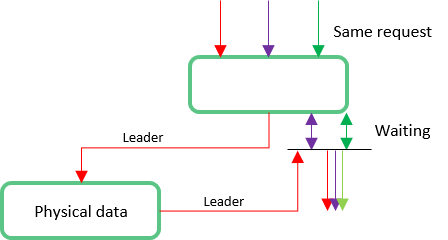
\includegraphics[width=0.8\linewidth]{img/loadwaiting}
\caption{\label{loadwaiting}Data processing of load waiting strategy.}
\end{figure}

Load waiting strategy is used to prevent multiple requests for requesting same data from the physical database at the same time. It is a kind of avoiding of resource wasting. Once hot-spot data miss and there are mass of requests flowing into database within a very short period time. The principle is to elect a leader to fetch data from database, others, requesting for data with the same key, will be suspended until the leader processed. Figure \ref{loadwaiting} shows the process of load waiting strategy.

The framework identify the same requests by the cacheKey, which is a unique identification for the data. Processing is a hash map storing the different processing requests. A request want to fetch the data from database, $DataHelper$ will search whether the same request is being processed. The framework try to get request from Processing hash map by cacheKey. If the result is null, it indicates that the request is a new request. In the concurrency, there are mass of the requests, the framework will select the first request as a leader to fetch data from physical data, others are waiting until the leader notify them and bring the data back. The speci?c load waiting strategy algorithm is as Algorithm \ref{loadwaitingalg}.

\begin{algorithm}
\caption{Load waiting strategy algorithm \textit{loadwaiting}}
\label{loadwaitingalg}
\begin{algorithmic}[1]
\REQUIRE ~~\\
  String $cacheKey$;\\
  Map $hashMap$;
\ENSURE ~~\\

\STATE Processing processing = hashMap.get(cacheKey);
\IF{processing == null}
\STATE Processing newProcessing = new Processing();
\STATE Processing \_processing = HashMap.putIfAbsent(cacheKey, newProcessing);
\IF{null != \_processing}
\STATE processing = \_processing
\ENDIF
\ENDIF

\IF{processing == null}
\STATE doRequest(newProcessing)
\STATE newProcessing.setFirstFinish(TRUE);
\STATE hashMap.remove(cacheKey);
\STATE newProcessing.notifyAll();
\ELSE
\STATE waitUntilLeaderGotData(processing);
\ENDIF


\RETURN

\medskip

\end{algorithmic}
\end{algorithm}

\subsubsection{Auto Loading Strategy}
Generally, each cache have its own expired time, which it's not suitable for high-frequent cache or time-consuming data in in-memory cache. Once expired, the system has to fetch those data from data source, which may consume lots of resources and make response slow. Therefore, those types of data should reside in the memory until they don't take too many resources when fetching them.

Figure \ref{autoloading} shows the management of the query autoloading queue. $hashTable$, which providing a method called $putIfAbsent$ to avoid duplicate tasks and controlling the number of auto load tasks, is a storage for auto load assignments. $taskQueue$ is taken from $hashTable$ by a unified strategy, like LRU. In distributed scenario, the standardized sequence of tasks help the system reduce the read back of source, because others can fetch data from cache rather than database after first server loaded. Auto load, however, is a double-edged, the system may become unstable if the amount of auto load tasks were too much or update frequency were too high. Accordingly, a strict inspection should be applied. We assume that $t_n$(ms) is current time, $t_{fr}$(ms) is the first request time, $t_{lr}$(ms) is last request time,  $t_a$(ms) is the average of fetching time, $c$ is the times of cache usage, $t_{to}$ is a preset parameter determining cache time out. There are three main aspects as follow:

\begin{itemize}
    \item Remove if the targeting cache is not requested for a long time. The time of not be requested is get from $t_{nr} = t_n - t_{lr}$, if $t_{nr} > t_{to}$, the task will be discarded.
    \item Remove if efficiency of fetching data from database is high. This may be confused. The intention of auto load is pre-load the data that cost a lot of time and resources and be accessed frequently. Hence, the data that obtaining efficiency is high should not occupy the space of auto load. The standard of determination is $c > 100$ and $t_a < 10$.
    \item Remove if usage rate is low. If the cache, which is requested only once within the preset timeout, were added to auto load queue, that will go against the purposes of auto load. Therefore, only removing the task that the targeting cache is not requested for a long time is not enough. The usage rate can be get from $r = \frac{c}{\frac{t_n - t_{fr}}{3600000}}$, the meaning of $r$ is how much the cache is requested per hours. If the task has been running for more than 1 hour and the average loading time is less than 1000 ms and $r$ is less than 60, the task will be removed.
\end{itemize}{}

The last part of auto load is when to refresh the cache. As a pre-loading schema, the cache should be refreshed before expired. For this reason, setting alarm time is valuable. Experiments prove that the default alarm time should be set $t_e - 120$ if $t_e \geq 600$ or $t_e - 60$ if $t_e < 600$, which $t_e$ is a preset parameter determining cache expired time.


\subsubsection{Cache Delete in Batches}
It is difficult to restore or obtain the cache key that need to delete when the query statements are complex, active deletion will hardly complete. In order to manage that, "namespace + hfield + cachekey" schema is proposed. The cache is added string, indicating its namespace, before the cache key, aiming to address conflict in the cache cluster. For active deletion, the key point is that establish a hash table to store the caches that need to be removed together. "hfield" is to identify a unique hash table. Developers can design the deletion granularity on need basis. The process of cache delete in batches is ACALFA intercepts the delete request and inspect whether hfield is set. If hfield is set, ACALFA will delete all the cache that store in corresponding hash table. If not, ACALFA will only delete that cache.

\subsection{Annotation}
Aspects at particular join points enable the modularization of concerns such as cache management that cut across multiple types and objects. We use interceptor as an advice in aspects. Cache pointcuts are put in all DAO classes to implement business hierarchy. Several annotations are designed to describe pointcuts. This framework need intercept the methods with cache annotation and apply cache strategy. There are several annotations, such as $@Cache$, $@ExCache$, $@CacheDeleteKey$, $@CacheDeleteTransactional$, and $@LocalCache$.

\subsubsection{Cache}
$@Cache$ that describes the entrance of in-memory caches is one of the most critical annotations. This cache framework will parse the cache configuration in $@Cache$ after intercepting this annotation, such as expiration time, the expression of the cache key. When the function of DAO returns data (the data is obtained from the physical database), the framework synchronize the data into the in-memory cache.

\subsubsection{ExCache}
$@ExCache$ implements generating multiple caches in one request. It is used to reduce the number of read back of source as long as sorting out the relationship between the cache. The implement of this feature is that framework will determine whether $@Cache$ contains $@ExCache$ items or not. If yes, framework will generate a new cache according to the configuration.

\subsubsection{CacheDelete}
$@CacheDelete$ and $@CacheDeleteKey$ implement the cache deleting strategy. $@CacheDelete$ is used to remove the cache. $@CacheDeleteKey$ is used to generate the cache key that will be removed. The structures are shown as Table \ref{CacheDelete} and \ref{CacheDeleteKey}.

\begin{table}[htb]
\begin{center}
 \caption{\label{CacheDelete}$CacheDelete$ annotation.}
 \begin{tabular}{lll}
 \toprule
Name & Type & Description\\
 \midrule
value & CacheDeleteKey[] & CacheDeleteKey array\\
\bottomrule
 \end{tabular}
\end{center}
\end{table}

\begin{table*}[htb]
\begin{center}
 \caption{\label{CacheDeleteKey}$CacheDeleteKey$ annotation.}
 \begin{tabular}{lll}
 \toprule
Name & Type & Description\\
 \midrule
condition & String & Condition expression and it will return true or false.\\ %The caches are deleted only when its return is true\\
value & String[] & An array saving the cache key expression\\
hfield & String & Expression of hash table field\\
\bottomrule
 \end{tabular}
\end{center}
\end{table*}

\subsection{Expression}
Expression language (EL) is used to generate dynamical variable in the annotation. For example, it can generate the cache key dynamically. There are many types of EL engine, such as Spring EL, Ognl, JavaScript EL. In the case of high performance requirement, Ognl is close to the primitive code. This cache framework provides an abstract class for developers to add user-defined EL.

\begin{itemize}
  \item $addFunction$ means adding a custom method. In the class of expression parser, there is a hash table which is named $customFunction$s. The key of $customFunctions$ is EL expression, and the value of that is a custom method. In this way, the relationship between expression and custom method is created.
  \item $getExpressionValue$. Converting an expression to an expected value. The parameters are shown in Table \ref{getExpressionValue}. This function traverses the keys in $customFunctions$ to register those custom functions.
\end{itemize}

\begin{table}[htb]
\begin{center}
 \caption{\label{getExpressionValue}Parameters of getExpressionValue.}
 \begin{tabular}{ll}
 \toprule
Name & Description\\
 \midrule
arguments & Parameters of intercepted method\\
retVal & Return value of intercepted method\\
hasRetVal & reVal is required or not\\
valueType & Return type of intercepted method\\
\bottomrule
 \end{tabular}
\end{center}
\end{table}

\section{Experiments}
\label{Experiments}

\subsection{Experiment Setup}
Three experiments are designed to illustrate the ACALFA performance in high-concurrency scenario. The metrics are response time, resource consumption and stability. Response time is for validating the optimization of auto load, especially for time-consuming tasks and high-frequent business. Resource consumption is for validating the load wait performance when handling the same requests. Stability testing uses multiple threads to access applications simultaneously to simulate high concurrency. The server with ACALFA is an Intel Core i7 @ 3.40GHz CPU, 16GB memory, and 100Mbps bandwidth, and this server runs a 64-bit Windows 10 with a Java 1.8 64-bit server JVM. Another server with MySQL database runs on Ali ECS Cloud Server: 2 core 2.60GHz Intel Xeon E5-2650 CPU machines with 4 GB RAM, 40GB SSD and 100 Mbps Ethernet. The system is CentOS 6.8 x64. Spring Cache, a well-known cache management framework at j2ee, will be compared with ACALFA for performance. The dataset, the structure is shown in Table \ref{VTS}, is selected 4,000 records randomly from a voting system.

\begin{table*}[htb]
\begin{center}
 \caption{\label{VTS}Voting Table Structure.}
 \begin{tabular}{lll}
 \toprule
    Field & Type & Description\\
 \midrule
    id & INT & primary key\\
    candidate\_id & INT & candidate identification\\
    voter\_id & INT & voter identification\\
    score & INT & candidate scores between 1, 100\\
\bottomrule
 \end{tabular}
\end{center}
\end{table*}

\subsection{Response Time}

We set up six experiments to test the ACALFA effect. Cache expired time we set was 120s and enabled auto load and load wait for ACALFA. Exp1, exp3 and exp5 used ACALFA, on the contrary, others used Spring Cache. The experiment sets are as follow:

\begin{itemize}
    \item Exp1 \& Exp2: The resources that will be requested were not in cache. Therefore, the frameworks should fetch data from database.
    \item Exp3 \& Exp4: The response time when cache hit.
    \item Exp5 \& Exp6: After exp1 and exp2 120s, in other words, cache expired, we send requests again for validating the effect of auto load.
\end{itemize}

\begin{figure} [htb]
    \centering
    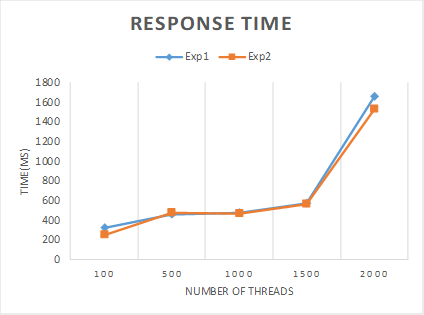
\includegraphics[width=1\linewidth]{img/exp1-2.png}
    \caption{Response time of Exp1 and Exp2}
    \label{exp1-2}
\end{figure}

\begin{figure} [htb]
    \centering
    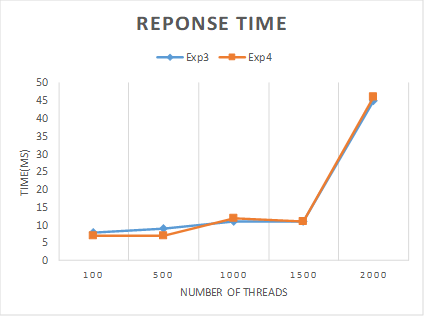
\includegraphics[width=1\linewidth]{img/exp3-4.png}
    \caption{Response time of Exp1 and Exp2}
    \label{exp3-4}
\end{figure}

\begin{figure} [htb]
    \centering
    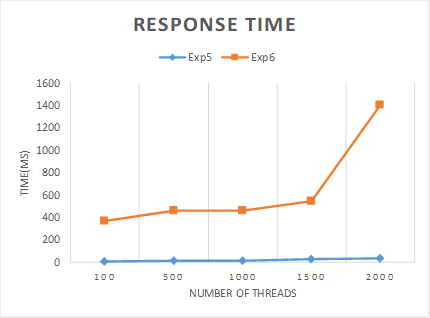
\includegraphics[width=1\linewidth]{img/exp5-6.png}
    \caption{Response time of Exp1 and Exp2}
    \label{exp5-6}
\end{figure}

We use the 90th percentile response time for performance measurement. Figure \ref{exp1-2} and figure \ref{exp3-4} shows the response time is increasing with the increase of number of threads. The performance of two cache management systems when cache miss or cache hit is same roughly. Figure \ref{exp5-6}, however, shows vast difference between ACALFA with auto load and Spring Cache. The reason is obviously: ACALFA will reload data when the cache is going to expire, but Spring Cache can't. According to this range of experiments, we found auto load is suited to the hot-spot data and has better cache effects for the more time-consuming or more frequent data.

\subsection{Resource Consumption}

Resource consumption experiment is set for validating the load wait performance. Therefore, the cache is disabled and the query statement is changed to join two tables for increasing cpu usage. There are 30 threads and request 10 times repeatedly. The CPU usage is shown in figure \ref{resource}. From results, CPU usage of non-load-wait lasted for a long time in 100\%. However, ACALFA selected a leader to fetch data in each round of request to reduce the CPU consumption. According to the results, we found wait-load strategy is effective in cache miss situation. Coordinate with auto-load, ACALFA can deal with complex and high-concurrent scenario well.

\begin{figure} [htb]
    \centering
    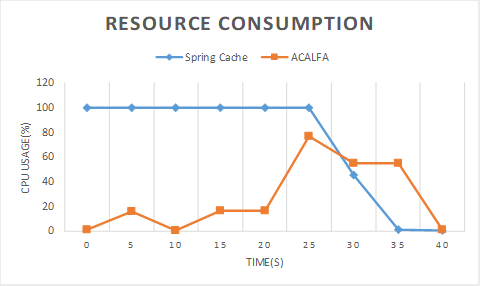
\includegraphics[width=1\linewidth]{img/resource.png}
    \caption{CPU usage of performing the select statement}
    \label{resource}
\end{figure}

\subsection{Pressure Test}

 \begin{figure}
     \centering
     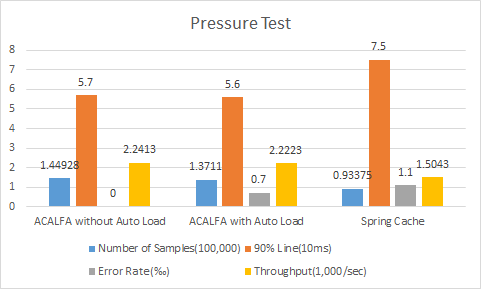
\includegraphics[width=1\linewidth]{img/pressuretest.png}
     \caption{Pressure with different methods}
     \label{pressuretest}
 \end{figure}

 The pressure test is getting access to a page repeatedly within one minute in order to test the stability of ACALFA in high concurrency. We used 100 threads to simulate 100 users for requesting the targeting page simultaneously. We can infer the system availability and response speed from the report. The query statement is same as resource consumption experiment. We can learn ACALFA response is 25\% faster than Spring Cache, processing speed is 48\% faster and stability has improved 36\% from above figure \ref{pressuretest}.

\section{Conclusions}
\label{Conclusions}
The purpose of a cache is to duplicate frequently accessed or important data in such a way that it can be accessed very fast and close to where it is needed. In the big data era, caching generally moves data from a low cost. This paper introduces an aspect-oriented cache auto load framework with annotation. Several experiments are illustrated that our cache framework has a good effect on the complex business with high concurrency. In the future work, memory resource cost will be optimized to increase cache hit ratio.


%\section*{Acknowledgement}
%The project is funded in part by the National Institutes of Health, under Grant No. 5R01CA136535.


%%%%%%%%%%%%%%%%%%%%%%%%%%%%%%%%%%%%%%%%%%%%%%%%%%%%%%%%%%%%%%%%%%%%%%%%%%%%%%%%%%%%%

%\bibliography{ijmso}
%\bibliographystyle{unsrt}
%\bibliographystyle{alpha}

\bibliography{mybibtex}
\bibliographystyle{unsrt}

\end{document}
